\chapter{Upper Bound}
\label{ch:rel-ent}

\textcolor{red}{denk nochmal \"uber die struktur hier nach, also mit den
numerischen approaches. naive approach zu den anderen? Auch auf simulations
chapter verweisen!}

In this chapter we explore the approach of
\citeauthor{garrattProbingPostmeasurementEntanglement2023} presented in
\cite{garrattProbingPostmeasurementEntanglement2024}. They introduce a method
to probe the critical point of the phase transition of a hybrid circuit. In
particular, they make use of Klein's inequality, bounding the entanglement
entropy from above. In the present chapter we introduce the idea behind this
approach, translate it to our system -- the projective transverse-field Ising
model (PTIM) --, and evaluate the quality of the resulting estimate. The
chapter is structured as follows. In \cref{sec:upperbound-idea} we state the
principles behind the idea and derive the upper bound. Moreover, we state and
prove that for Clifford circuits, i.e. in the stabilizer formalism, there is
only a limited class of cases, where the upper bound is non-trivial. In
\cref{sec:upperbound-numerics} we introduce different numerical post-processing
algorithms, trying to combat infinities appearing, when introducing an error
model akin to the one in \cref{sec:lxe-errors}. The results of which are shown
and discussed in \cref{sec:upperbound-results}. Finally, we provide and discuss
regularizations of divergences, weighing out utility and
computational efficiency.

%computable quantities
%In this chapter we investigate if Klein's Inequality can assist us in obtaining
%a sensible upper bound for the entanglement entropy and thus make the
%entanglement transition visible.
%
%Idea from Altman Paper:
%\citetitle{garrattProbingPostmeasurementEntanglement2023}
%\cite{garrattProbingPostmeasurementEntanglement2023}.
%In \cite{garrattProbingPostmeasurementEntanglement2023} they introduce a method
%to obtain an upper bound on the entanglement entropy via classical
%post-processing.
%
\section{The Idea \& Stabilizers}\label{sec:upperbound-idea}
In this section we will introduce the upper bound on entanglement entropy,
provide an information-theoretic interpretation and derive an expression for
the quantity of interest in case of stabilizer states. First however, we will
freshen up on definitions of some important quantities.
\subsubsection{Entropy of entanglement}
The main quantity of interest in the whole field of entanglement transitions is
the entropy of entanglement. It is a measure for how entangled one subsystem of a
bipartite state $\ket{\phi}_{AB}$ is with the other. We recall from
\cref{sec:ent-trans} that its definition can be stated as follows
\cite{fattalEntanglementStabilizerFormalism2004}.
\begin{defn}[Entanglement entropy]\label{defn:entanglement-entropy}
  Let $\ket{\phi}\in H^{\otimes N}$ be a bipartite pure state with subsystems
  $A$ and $B$. The entropy of entanglement of $\ket{\phi}$ then reads
  \begin{align}
    %&S_E : H^{\otimes N} \to [0, N/2]\nonumber\\
    S_\mathrm{E}\left(\ket{\phi}\right) \equiv - \Tr[\rho_B \log \rho_B],
  \end{align}
  where $\rho_B = \Tr_A[\dyad{\phi}]$ is the reduced density matrix of subsystem
  $B$. Conventionally, one uses the logarithm of base 2.
\end{defn}
This quantity can be efficiently computed in clifford circuits via the
stabilizer formalism. It is important to note that the density matrix of the
whole system $\rho = \dyad{\phi}$ describes a pure state. For a more universal
measure of entropy, where the entropy of entanglement is a special case, we
need to consider the more general \emph{von Neumann entropy}.
\subsubsection{Von Neumann entropy}
The von Neumann entropy lets us quantify the average information content in a mixture of
quantum states. Originally, von Neumann introduced it as an extension of the
classical Shannon entropy to quantum systems, as density matrices serve as
extension of the classical notion of (discrete) probability distributions
\cite{vonneumannMathematischeGrundlagenQuantenmechanik1968}.\footnote{Shannon
  entropy is a measure of the average information of probabilistic events.
  Since Information is defined as $I=-\log p_x$ for some event $x$ with
  probability $p_x$, we can write down an average, $S = \expval{-\log p_x}_x =
  -\sum_x p_x \log p_x$, which defines the Shannon entropy
\cite{shannonMathematicalTheoryCommunication1948}.} 
Consequently, we can write down a definition of the von Neumann entropy.
\begin{defn}[Von Neumann entropy]\label{defn:vonneumann}
  Let $\rho$ be an $N$-qubit density matrix. The von Neumann entropy of $\rho$
  is given by
  \begin{align}\label{eq:entropy-vn}
    S\left(\rho\right) \equiv \expval{-\log \rho} = -\Tr[\rho\log\rho]
  .\end{align}
\end{defn}
For diagonalizable matrices (as we expect density matrices to be) we can also
express \cref{eq:entropy-vn} as a sum over eigenvalues $\lambda_k$ of $\rho$, i.e.
\begin{align}\label{eq:entropy-vn-sum}
  S\left(\rho\right) = -\sum_k \lambda_k \log \lambda_k
,\end{align}
where $0\leq\lambda_k\leq 1$.
This can be shown by diagonalizing $\rho$ and using the fact that the matrix
logarithm of a diagonal matrix is just the logarithm of the entries.
(Note that we set $0\cdot\log 0 \equiv 0$.)

From this definition we can already derive some important properties, namely
its lower and upper bound. Firstly, $S(\rho)$ is non-negative and $0$ iff.
$\rho$ is pure. It is easy to convince oneself of that fact; for pure states we
have $\rho = \dyad{\phi}$, which has only one non-zero eigenvalue, $\lambda =
1$. Consequently, \cref{eq:entropy-vn-sum} reduces to $S(\rho) = - 1\cdot\log 1
=0$.  Next, $S(\rho)$ is maximal for the maximally mixed state. In a
$d$-dimensional Hilbert space, the density matrix of the maximally mixed state
is $\rho = \mathds{1}/d$. Hence, \cref{eq:entropy-vn-sum} reduces to
\[
  -\sum_k \frac{1}{d} \log \frac{1}{d} = -\log \frac{1}{d} = \log d
.\]
%One property we want to emphasize in particular is that $S(\rho)$ is bounded
%from above and below; it is $0$ for a pure state and $\log d$ for a maximally
%mixed state in a $d$-dimensional Hilbert space.
\subsubsection{Quantum relative entropy}
Lastly, we want to introduce the quantum relative entropy. 
%In classical
%information theory the relative entropy of one probability distribution $p_x$
%to another distribution $q_x$ provides a measure of excess information.
%Lost in the sense that if one assumes $q_x$ as the probability distribution
%over some sample space, where 
The same way we
motivated the von Neumann entropy, we want to define a quantum mechanical
analogue to the classical relative entropy. This quantity will play a role of
major importance in this chapter and is defined as follows.
\begin{defn}[Quantum relative entropy]\label{defn:rel-ent}
  Let $\rho$ and $\sigma$ be density matrices with identical dimension. The
  relative entropy of $\rho$ to $\sigma$ is
  %$S: H^{\otimes N} \times H^{\otimes N} \to \mathbb{R}^+_0 \cup \{\infty\}$
  \begin{align}\label{eq:rel-ent-defn}
    S\left(\rho\mid\mid\sigma\right) \equiv \Tr[\rho\log\rho] -
    \Tr[\rho\log\sigma] = -S(\rho) - \Tr[\rho\log\sigma]
  ,\end{align}
  with the von Neumann entropy $S(\rho)$.
  The last term in \cref{eq:rel-ent-defn}, that is, $\Tr[\rho\log\sigma]$ is also
  known as \emph{cross entropy}. 
\end{defn}
Relative entropy, classical or quantum, quantifies excess surprisal when
one assumes $\sigma$ as a state\footnote{or probability distribution in the
classical case}, when the actual state is $\rho$. In that sense it tells us how
different two quantum states are. Interpreting it in this way also provides us
with a neat heuristic approach to possible values: the only way we do not lose
information is if we assume correctly, and in any other case we lose some. The
most extreme form of this is if $\mathrm{supp}(\rho)\cap\mathrm{ker}(\sigma)={0}$, where the
relative entropy diverges. In most general terms the relative entropy fulfils
\begin{align}\label{eq:inf-cond}
  S(\rho\mid\mid\sigma) < \infty \Longleftrightarrow \mathrm{supp}(\rho) \subseteq
  \mathrm{supp}(\sigma)
,\end{align}
where supp$(\bullet)\equiv\ $ker$(\bullet)^\perp$ is the support of a linear
operator, which is defined as the orthogonal complement to the kernel.
Alternatively, for diagonalizable matrices, it is the subspace spanned by
eigenvectors with non-zero eigenvalues
\cite{leditzkyRelativeEntropiesTheir2016,schumacherRelativeEntropyQuantum2000}.
This condition can be interpreted in a physical way. Let
\[
  \rho = \sum_i \lambda_i \dyad{\lambda_i} \quad{\text{and}} \quad
  \sigma = \sum_i \mu_i \dyad{\mu_i}
\]
be orthonormal eigendecompositions of $\rho$ and $\sigma$.
Then $S(\rho\mid\mid\sigma)$ diverges iff. there are states that $\rho$
features in its mixture that $\sigma$ doesn't. That is, $\rho$ has to be more
mixed than, or at least as mixed as, $\sigma$. If it is as mixed as
$\sigma$, it has to be a mixture of the same states. This means that the
information lost under the assumption of a purer state is infinite.
Since we know the von Neumann entropy to be bounded, this divergence occurs
solely in the $-\Tr[\rho\log\sigma]$ term. 

One property hinted at earlier is the non-negativity of the relative entropy.
This property goes by many different names, depending on context. For instance,
in classical statistical mechanics, this result is known as the \emph{Gibbs
inequality}. Its quantum mechanical analog is also known as \emph{Klein's
inequality}.
\subsection{Klein's inequality}
In this section we will state and prove the relation central to this chapter.
Its statement reads as follows.
\begin{thm}[Klein's inequality]\label{thm:kleins-ineq}
  The quantum relative entropy is non-negative, $S(\rho\mid\mid\sigma)\geq 0$, with equality iff.
  $\rho=\sigma$.
\end{thm}
While the statement in itself is written out rather simply, proving
\cref{thm:kleins-ineq} requires
us to introduce two auxilliary relations, namely \emph{Jensen's inequality} and
the \emph{log sum inequality}.
%Before we can go about proving \cref{thm:kleins-ineq}, we first need to
%introduce two auxilliary statements, which will be proven in the following.
%non-negativity of the classical relative entropy first. To this end, we introduce and
%prove some auxilliary lemmata, beginning with Jensen's inequality.
\begin{thm}[Jensen's inequality]\label{thm:jensen}
  Let $f$ be a convex function, that is, $f\left(\lambda x_1 + \left(
  1-\lambda \right)x_2\right) \leq \lambda f\left( x_1 \right) + \left(
  1-\lambda \right) f(x_2)$ with $0\leq\lambda\leq1$, and $X$ a discrete random
  variable. Then
  \begin{align}
    \mathbb{E}\left[f(X)\right] \geq f\left( \mathbb{E}\left[X\right] \right)
  .\end{align}
\end{thm}
\begin{proof}[Proof of Jensen's inequality]
  We will prove Jensen's inequality by induction over the mass of $X$.
  Associated with each event $x_i \in X$ is its probability $p_i$, such that
  our induction hypothesis is
  \begin{align}\label{eq:ind-hyp}
    \sum_{i=1}^n p_i f\left(x_i\right) \geq f\left(\sum_{i=1}^n p_i x_i
    \right).
  \end{align}
  As base case we have $n=2$;
  \begin{alignat*}{2}
    \mathbb{E}\left[f(X)\right] 
      &= p_1 f(x_1) + p_2 f(x_2) \\
      &= p_1 f(x_1) + (1-p_1) f(x_2) &&\qquad{\text{(Kolmogorov)}}\\
      &\geq f(p_1x_1 + (1-p_1)x_2) &&\qquad{(f\text{ convex})}\\
      &= f(\mathbb{E}[X])
  .\end{alignat*}
  For the induction step, assume \cref{eq:ind-hyp} holds for some
  $n\in\mathbb{N}_{>1}$, it must then also hold for $n+1$;
  \begin{alignat*}{2}
    \sum_{i=1}^{n+1} p_i f(x_i) 
      &= p_{n+1} f(x_{n+1}) + \sum_{i=1}^n p_i f(x_i)\\
      &= p_{n+1} f(x_{n+1}) + (1-p_{n+1})\sum_{i=1}^n \frac{p_i}{1-p_{n+1}} f(x_i)\\
      &\geq p_{n+1} f(x_{n+1}) + (1-p_{n+1})f\left(\sum_{i=1}^n
  \frac{p_i}{1-p_{n+1}} x_i\right) &&\qquad{\text{(Induction hypothesis)}}\\
      &\geq f\left(p_{n+1}x_{n+1} + (1-p_{n+1})\sum_{i=1}^n \frac{p_i}{1-p_{n+1}} x_i\right)
      &&\qquad{(f\text{ convex})}\\
      &=f\left(\sum_{i=1}^{n+1}p_i x_i\right).
  \end{alignat*}
  Since the base case and the induction step hold, we conclude that it holds
  $\forall n \in \mathbb{N}_{>1}$.
\end{proof}
\begin{cor}[Log sum inequality]\label{cor:logsum}
  Let $a_1, \ldots, a_n, b_1, \ldots, b_n \geq 0$ and let $a = \sum_i a_i$ and
  $b = \sum_i b_i$. Then
  \begin{align}\label{eq:logsum}
    \sum_{i=1}^n a_i \log \frac{a_i}{b_i} \geq a \log \frac{a}{b}
  .\end{align}
\end{cor}
\begin{proof}
  Let $f(x)=x\log x$. It is easy to convince oneself that $f$ is convex, and
  that it lets us rewrite the left side of \cref{eq:logsum}. We then have
  \begin{alignat*}{2}
    \sum_i a_i \log \frac{a_i}{b_i}
      &=\sum_i b_i f\left( \frac{a_i}{b_i} \right) 
      =b\sum_i \frac{b_i}{b} f\left( \frac{a_i}{b_i} \right) \\
      &\geq b\cdot f\left( \sum_i \frac{b_i}{b}\frac{a_i}{b_i} \right)
      &&\qquad{\text{(\cref{thm:jensen})}}\\
      &= b\cdot f\left( \frac{1}{b}\sum_i a_i \right)
      = b\cdot f\left( \frac{a}{b}\right) \\
      &= a \log \frac{a}{b}
  .\end{alignat*}
%  We can apply Jensen's inequality, since $\sum_i \frac{b_i}{b} = 1$ can be
%  taken as an average.   
\end{proof}
%Before we state the proof of \cref{thm:kleins-ineq} 
We now have all the tools ready to prove \cref{thm:kleins-ineq}. Our proof
follows the one laid out in \cite{nielsenQuantumComputationQuantum2010}, with
slight modifications.
\begin{proof}[Proof of \cref{thm:kleins-ineq}]
  Let $\rho=\sum_i p_i \dyad{i}$ and $\sigma=\sum_j q_j \dyad{j}$ be
  orthonormal decompositions for $\rho$ and $\sigma$. From \cref{defn:rel-ent}
  we can write
  \begin{align}\label{eq:ke-proof1}
    S(\rho\mid\mid\sigma) = \sum_i p_i \log p_i - \sum_i \bra{i} \rho
    \log\sigma \ket{i}
  .\end{align}
  With the eigendecomposition of $\rho$ and $\sigma$ we can write $\bra{i} \rho = p_i
  \bra{i}$ and
  \begin{align}\label{eq:ke-proof2}
    \expval{\log\sigma}{i} = \expval{\left(\sum_j \log q_j \dyad{j}
    \right)}{i} = \sum_j P_{ij}\log q_j  
  ,\end{align}
  with $P_{ij} = \ip{i}{j}\ip{j}{i} \geq 0$. 
  Plugging this into \cref{eq:ke-proof1} yields
  \begin{align}\label{eq:ke-proof3}
    S(\rho\mid\mid\sigma) = \sum_i p_i \left(\log p_i - \sum_j P_{ij} \log q_j \right)
  .\end{align}
  Note that $P_{ij}$ satisfies $\sum_i P_{ij} = \sum_j P_{ij} = 1$. We can thus
  interpret the last term in \cref{eq:ke-proof3} as an average of $-\log q_j$.
  Since $-\log$ is a strictly convex function it follows from \cref{thm:jensen}
  that
  \begin{align}
    -\sum_j P_{ij} \log q_j \geq - \log r_i
  ,\end{align}
  where $r_i = \sum_j P_{ij} q_j$, with equality iff. there exists a value of
  $j$ where $P_{ij}=1$. This implies 
  \begin{align}
    S(\rho\mid\mid\sigma) \geq \sum_i p_i \log\frac{p_i}{r_i}
  ,\end{align}
  where the equality occurs iff. there exists a $j$ with $P_{ij}=1$, i.e. iff.
  $P_{ij}$ is a permutation matrix.

  By \cref{cor:logsum} and the double stochasticity of $P_{ij}$ we obtain the
  final result
  \begin{align}
     S(\rho\mid\mid\sigma) \geq \sum_i p_i \log\frac{p_i}{r_i} \geq 1\cdot \log
     \frac{1}{1} = 0
  .\end{align}
\end{proof}

This result is essentially already our upper bound on the entanglement entropy,
since we have
\begin{align}
  \label{eq:kleins-ineq}
  S(\rho \mid\mid \sigma) \geq 0 \Leftrightarrow -\Tr[\rho\log\sigma]\geq
  S\left( \rho \right) 
\end{align}
with the relative and von Neumann entropy $S(\rho\mid\mid\sigma)$ and
$S(\rho)$ respectively. Since the von Neumann entropy is a more general form of
the entanglement entropy, we can employ Klein's inequality to upper bound the
entanglement entropy as well and thus try to find a signature of the phase
transition.

This idea was used in \cite{garrattProbingPostmeasurementEntanglement2024} for
a hybrid circuit of Haar random 2-qubit unitaries and $Z$ measurements. Since
they investigate a hybrid circuit, they take additional steps to circumvent the
post-selection problem, such as shadow tomography. To test their approach they
simulate their circuits with matrix product state (MPS) simulations. These
allow for a broader spectrum of mixed states than stabilizers do, and it is
computationally expensive, but feasible, to diagonalize the density matrix and
take its logarithm, to then compute the cross entropy upper bound. In our case,
however, we investigate a random circuit consisting of pauli measurements only
and thus employ stabilizer simulations to run numerical experiments on a
classical computer. As already elaborated on in \cref{sec:stab-basics},
the stabilizer formalism allows for lots of elegant computational shortcuts,
allowing efficient quantum simulations on classical computers. Consequently,
one might ask if there also is an efficient way to compute the cross or
relative entropy. We will explore this question in the next section.

%Among other things, they make use of shadow tomography to circumvent the
%post-selection problem. 
%However, they do MPS simulations, and not stabilizer. This, of course, calls
%for an adaptation (oh well\ldots).
%\begin{itemize}
%  \item \cite{garrattProbingPostmeasurementEntanglement2024} do mps
%    simulations, which, as it turns out, have a broader spectrum of mixed states than stabilizer
%    states. 
%  \item thats why they need shadow tomography and stuff
%  \item also, they do a hybrid circuit with random haar unitaries
%  \item only one type of measurement and the probability refers to if any
%    measurement is performed (on the computational basis)
%  \item MPS has lower dimensions, it is computationally expensive, but
%    feasible, to diagonalize the density matrix and take its log
%  \item[$\to$] what about clifford circuits? is there a way to write out the
%    relative entropy for stabilizers? In fact, there is:
%\end{itemize}


\subsection{Stabilizers}\label{sec:rel-ent-stab}
In this section we will investigate the upper bound on the entanglement entropy
given by \cref{thm:kleins-ineq} in the context of stabilizers and the
stabilizer formalism. In particular, we will explore the condition of infinite
relative entropy,
provide and prove a necessary and sufficient condition
for $S(\rho\mid\mid\sigma)<\infty$ when $\rho$ and $\sigma$ are stabilizer
density matrices (\cref{prop:subgroup}), and derive an expression for finite cross
and relative entropy.

Recall that we have $S(\rho\mid\mid\sigma)<\infty$ for
supp$(\rho)\subseteq$supp$(\sigma)$. For the proof of \cref{prop:subgroup} it
will prove useful to introduce an auxilliary lemma, which relates the support
of a density matrix to the stabilized subspace.
\begin{lem}\label{lem:supp-is-vs}
  Let $\rho$ be an $N$-qubit stabilizer density matrix with stabilizer group $S = \langle
  g_1, \ldots, g_n \rangle$, and $0\leq n \leq N$.
  Then \[ \mathrm{supp}(\rho) = V_{S}.\]
\end{lem}
\begin{proof}[Proof of \cref{lem:supp-is-vs}]
  By definition (cf. \cref{ch:basics}) we take $V_{S}$ to be the vector space
  stabilized by $S$.  Further, it is the intersection of subspaces fixed by
  each operator in $S$, i.e. the eigenvalue one eigenspaces of elements of $S$
  (cf.  \cref{ch:basics} and \cite{nielsenQuantumComputationQuantum2010}). More
  formally we can write
  \[ 
    V_S = \bigcap_{g \in S}  \left\{\ket{\psi} \mid g\ket{\psi} =
    \ket{\psi}\right\} = \left\{\ket{\psi} \mid g\ket{\psi} =
    \ket{\psi} \forall g \in S\right\}.
  \]
  This subspace is projected onto by
  \[ P_S \equiv \frac{1}{2^n} \prod_{g\in S} \left(\mathds{1} + g\right).\]
  Note that $\rho$ can be constructed from a product of projectors
  \cite{gottesmanStabilizerCodesQuantum1997}
  \[ \rho = \frac{1}{2^N} \prod_{g \in S} \left(\mathds{1} + g\right) = 2^{n-N} P_S \]
  We thus have
  \[ \mathrm{supp}(\rho) = \mathrm{supp}(P_S) = V_S. \]
\end{proof}

\begin{thm}\label{prop:subgroup}
  Let $\rho$ and $\sigma$ be $N$-qubit stabilizer density matrices with
  respective stabilizer groups $S_\rho$ and $S_\sigma$. Then
  \[ \mathrm{supp}(\rho)\subseteq \mathrm{supp}(\sigma) \Longleftrightarrow
  S_\sigma \leq S_\rho. \]
  That is, with \cref{eq:inf-cond}, $S(\rho\mid\mid\sigma)$ takes on finite values iff. $S_\sigma$ is a
  subgroup of $S_\rho$.
\end{thm}

\begin{proof}[Proof of \cref{prop:subgroup}]
  We will prove implication from both directions to prove equivalence.

  \enquote{$\Leftarrow$} Let $S_\sigma \leq S_\rho$. Then
  \begin{align*}
    \mathrm{supp}(\rho) = V_{S,\rho} &= \bigcap_{g\in S_\rho} \left\{ \ket{\psi} \mid
    g\ket{\psi} = \ket{\psi} \right\} \\
        &\overset{S_\sigma \leq S_\rho}{=} \underbrace{\bigcap_{g\in S_\sigma}
        \left\{\ket{\psi} \mid g \ket{\psi} =
        \ket{\psi}\right\}}_{V_{S,\sigma}}\ \ \ \cap \bigcap_{g \in S_\rho \setminus
        S_\sigma} \left\{\ket{\psi} \mid g \ket{\psi} =
        \ket{\psi}\right\}\\
        &= V_{S,\sigma} \cap \bigcap_{g \in S_\rho \setminus
        S_\sigma} \left\{\ket{\psi} \mid g \ket{\psi} =
        \ket{\psi}\right\}\\
        &\subseteq V_{S,\sigma} = \mathrm{supp}(\sigma)
  .\end{align*}
  which finishes the proof of this direction.

  \enquote{$\Rightarrow$} Let $V_{S,\rho} = \mathrm{supp}(\rho) \subseteq
  \mathrm{supp}(\sigma) = V_{S,\sigma}$. 
  For the proof of this direction, consider the relations between the subspaces
  of the $N$-qubit Hilbert space $H^{\otimes N}$ outlined in the following
  diagram.
  \begin{figure}[h]
    \centering
  \begin{tikzpicture}
  \matrix (m) [matrix of math nodes,row sep=3em,column sep=4em,minimum width=2em]
  {
    H^{\otimes N} & V_\rho \\
     V_\sigma &  \\};
  \path[-stealth]
    (m-1-1) edge node [left] {$P_\sigma$} (m-2-1)
            edge node [above] {$P_\rho$} (m-1-2)
    (m-2-1) edge node [below] {$P_\rho$} (m-1-2);
  \end{tikzpicture}
\end{figure}

  We can read the diagram as follows: From the $N$-qubit Hilbert space we can
  project onto the vector space stabilized by $S_\sigma$, $V_\sigma$, by means of a
  projection operator. Likewise we can do the same for $V_\rho$. Since we
  require $V_{S,\rho} \subseteq V_{S,\sigma}$, the same projection that takes
  us from $H^{\otimes N}$ to $V_{S,\rho}$ will take us from $V_{S,\sigma}$ to
  $V_{S,\rho}$. It follows that $P_\sigma P_\rho = P_\rho$.

  Let $\ket{\psi} \in V_\rho$. We thus have
  \[
    \ket{\psi} = P_\rho \ket{\psi} = P_\sigma P_\rho \ket{\psi} = P_\sigma
    \ket{\psi}.
  \]
  Since $\ket{\psi}$ was an arbirtary element from $V_{S,\rho}$ and $P_\sigma =
  \frac{1}{2^n} \prod_{i=1}^n \left(\mathds{1} + h_i\right)$ with $h_i \in
  S_\sigma$ it follows that all stabilizers of $\sigma$ also stabilize $\rho$
  and thus
  \[
    S_\sigma \leq S_\rho.
  \]
%  $\ket{\psi} \in V_{S,\rho}$ and $\ket{\phi} \in
%  V_{S,\sigma} \setminus
%  V_{S,\rho}$. \"o Since the stabilizer group is the
%  symmetry group of $V_S$, we can rewrite $S_\sigma$ as
%  \[ 
%    S_\sigma = \left\{ g \in G_N \mid g \ket{\psi} = \ket{\psi} \wedge g\ket{\phi} =
%  \ket{\phi} \right\},
%  \]
%  (where $G_N$ is the $N$-qubit Pauli group) 
%  as we want $S_\sigma$ to stabilize both $V_{S,\sigma}$ and its subset
%  $V_{S,\rho}$. We can then split up the condition into the intersection of two
%  sets, i.e.
%  \begin{align*}
%    S_\sigma &= \left\{ g \in G_N \mid g \ket{\psi} = \ket{\psi} \wedge g\ket{\phi} =
%  \ket{\phi} \right\}\\
%             &= \underbrace{\left\{ g \in G_N \mid g\ket{\psi}= \ket{\psi}
%             \right\}}_{S_\rho} \cap \left\{ g \in G_N \mid g\ket{\phi} = \ket{\phi} \right\} \\
%             &= S_\rho \cap \left\{ g \in G_N \mid g\ket{\phi} = \ket{\phi} \right\} \\
%               &\leq S_\rho 
%  .\end{align*}
  This concludes the proof.
\end{proof}
We have thus shown that that the condition for finite values of the relative
entropy is equivalent to a simple statement about the group structure of the
respective stabilizer groups. Furthermore, we know from 
\cite{fattalEntanglementStabilizerFormalism2004} that the entropy of
entanglement can be expressed in a simple way through group properties.
We'd like for this to also be the case for other entropic quantities,
especially the cross and relative entropy, which are our main concern.

It turns out that one can indeed derive expressions for the cross and relative
entropy that put these information-theoretic quantities in a relation with
abstract group properties. Confer with
\cref{thm:cross-ent-stab,col:rel-ent-stab} for the precise statements. The
resulting expressions are remarkable in their simplicity, as well as their
similarity to each other and to previous results. As a warm-up for the proofs
of \cref{thm:cross-ent-stab,col:rel-ent-stab} we will derive an expression for
the von Neumann entropy in the stabilizer formalism first. This will also aid
in the derivation of the expression for relative entropy, since it is a
difference of the cross and von Neumann entropy.

\begin{lem}[Von Neumann entropy -- stabilizers]\label{lem:vn-ent-stab}
  Let $\rho$ be an $N$-qubit stabilizer density matrix with stabilizer group
  $\mathcal{S}_\rho$ and rank $\abs{\mathcal{S}_\rho} \equiv r$. Then
  \begin{align}
    S\left( \rho \right) = N - r
  .\end{align}
\end{lem}
\begin{proof}
  Let $\mathcal{S}_\rho$ be an $N$-qubit stabilizer group of rank $r$ with
  corresponding density matrix $\rho$.

  By \cref{defn:vonneumann}, or \cref{eq:entropy-vn-sum} in particular, we have
  \begin{align}\label{eq:entropy-vn-sum-proof}
    S\left( \rho \right) = -\Tr[\rho\log\rho] = -\sum_k \lambda_k \log
    \lambda_k
  .\end{align}
  Thus, we need to diagonalize, i.e. find the eigenvalues $\lambda_k$ of
  $\rho$.

  Since $\rho$ is a stabilizer density matrix, it can -- up to a constant
  multiple -- also be written as a
  product of projectors onto the $+1$ eigenspaces of group generators
  \begin{align}
    \rho = \frac{1}{2^N} \prod_{i=1}^r (\mathds{1} + g_i) = 2^{r-N} \mathbb{P}_\rho
  .\end{align}
  Knowing that projections are diagonalizable with eigenvalues of either $0$ or
  $1$, we know that the diagonal form of $\rho$ is the diagonal form of
  $\mathbb{P}_\rho$ with a constant multiple $2^{r-N}$, that is\footnote{Note that
    the bottom right entry need not be zero. This specific choice was made for
  illustratory purposes.}
  \begin{align}
    D_\rho = 2^{r-N} \mqty(\dmat{1,\ddots,0})
  .\end{align}
  With $\Tr[\rho] = 1$ it follows that the eigenvalues of $\rho$ must be
  $\lambda_k = 2^{r-N}$ for $k =1,\ldots,2^{N-r}$ and
  $\lambda_k = 0$ for all other $k$.
  Inserting this back into \cref{eq:entropy-vn-sum-proof} yields
  \begin{align*}
    S\left( \rho \right) 
      &= -\sum_{k=1}^{2^N} \lambda_k \log \lambda_k 
      = -\sum_{k=1}^{2^{N-r}} 2^{r-N} \log 2^{r-N} 
      = -2^{N-r} 2^{r-N} \log 2^{r-N} 
      = -\log 2^{r-N} \\
      &= N-r
  .\end{align*}
\end{proof}
The expression of the von Neumann entropy is not only interesting going
forward, e.g. in the derivation of the relative entropy, but also from a group
theoretic perspective. That is, it should be noted that by asking an
information-theoretic question, we got a group theoretic answer. Let us
convince ourselves that it is a reasonable one, by testing it on our intuition
on entropy.

With $N$ qubits we have a generating set of size $N$, at most. In the case
where we have $N$ generators, the state associated with the stabilizer group is
a pure state, and the entropy should be $0$, which is the case for $r=N$. For
the maximally mixed state, the generating set is the empty set and the
stabilizer group the trivial group. In accordance to our expectations, this
should yield $\log(2^N)= N$ for the von Neumann entropy. Indeed, since the size of
the empty set is $0$, we have that $r=0$ and thus $S(\rho) = N$.

Removing one generator thus increases entropy by $1$, or put differently,
starting from the empty set and adding generators to it decreases entropy by
$1$ for each generator added. This too should come to no surprise, as we know
that for each generator removed (added) from a full set of stabilizers, we
double (halve) the stabilized state space, effectively creating (purifying) a
perfect mixture of stabilized states.

\begin{thm}[Cross entropy -- stabilizers]\label{thm:cross-ent-stab}
  Let $\rho$ and $\sigma$ be $N$-qubit stabilizer density matrices with
  respective stabilizer groups $S_\rho$ and $S_\sigma$ that satisfy $S_\sigma \leq
  S_\rho$. Further, let $\abs{S_\sigma} \equiv s$. Then
  \begin{align}\label{eq:cross-ent-stab}
    -\Tr[\rho\log\sigma] = N - s
  .\end{align}
\end{thm}

\begin{proof}
   Let $\mathcal{S}_\rho$ and $\mathcal{S}_\sigma$ be $N$-qubit stabilizer
   groups that satisfy $\mathcal{S}_\sigma \leq \mathcal{S}_\rho$. Their
   respective density matrices can be written as
   \begin{align}
     \rho = \frac{1}{2^N} \prod_{i=1}^r (\mathds{1} + g_i) \quad{\text{and}}
       \quad \sigma \frac{1}{2^N} \prod_{i=1}^s (\mathds{1} + h_i)
   \end{align}
   with $r \equiv \abs{\mathcal{S}_\rho}$ and $s \equiv
   \abs{\mathcal{S}_\sigma}$. Since we require $\mathcal{S}_\sigma \leq
   \mathcal{S}_\rho$, we can construct a generating set $G_\sigma$ of
   $S_\sigma$, where each element of $G_\sigma$ commutes with the generating
   set of $G_\rho$. Note that the generating sets are not necessarily
   identical. However, since $\mathcal{S}_\sigma$ is by construction a subgroup
   of $\mathcal{S}_\rho$, which in turn is an abelian subgroup of
   $\mathcal{P}_N$, all elements of $\mathcal{S}_\sigma$ commute with all elements of
   $\mathcal{S}_\rho$. It follows that the density matrices themselves also
   commute, i.e.
   \begin{align}
      \left[\rho, \sigma\right] = 0
   .\end{align}
   It is a well-known fact from linear algebra and functional analysis that
   commuting operators share a common eigenbasis and can be diagonalized
   simultaneously. We therefore write $\rho = UD_\rho U^{-1}$ and $\sigma =
   UD_\sigma U^{-1}$ with transformation matrix $U$ and corresponding diagonal
   matrix $D_{\rho / \sigma}$. We also have that the logarithm of a diagonalizable
   matrix is \cite{hallElementaryIntroductionGroups2000}
   $$\log \sigma = U \log D_\sigma U^{-1}.$$ Consequently,
   \begin{align}
      -\Tr[\rho \log\sigma] = -\Tr[U D_\rho U^{-1} U \log D_\sigma U^{-1}] =
      -\Tr[D_\rho \log D_\sigma] 
   .\end{align}
   With $D_\rho$ and $D_\sigma$ diagonal we can write the trace as
   \begin{align}\label{eq:the-sum}
      -\Tr[D_\rho \log D_\sigma] = -\sum_k \lambda_k \log \mu_k
   \end{align}
   with the eigenvalues $\lambda_k$ and $\mu_k$ of $\rho$ and $\sigma$,
   respectively.

   As we know from the previous proof, $\lambda_k = 2^{r-N}$ for
   $k=1,\ldots,2^{N-r}$ and $0$ otherwise, and analogously, $\mu_k = 2^{s-N}$
   for $k=1,\ldots,2^{N-s}$ and $0$ otherwise. Note that the subgroup condition
   implies that $r\geq s$ or more specifically $N-r \leq N-s$. This ensures that to every non-zero entry in
   $D_\rho$ there is a corresponding non-zero entry in $D_\sigma$. In other
   words, for all $k$, $\lambda_k \neq 0 \Rightarrow \mu_k \neq 0$. More
   importantly for us, however, is the contrapositive, $\mu_k = 0 \Rightarrow
   \lambda_k = 0$, which tells us that any divergence that might occur
   in the logarithm gets intercepted by a leading factor of $0$.

   Inserting this into the sum in \cref{eq:the-sum} we get
   \begin{align}
      -\sum_i 2^{r-N} \log 2^{s-N} =
      -2^{N-r}2^{r-N}\left(s-N\right)= N-s
   ,\end{align}
   which concludes the proof.
\end{proof}

Although \cref{thm:cross-ent-stab,eq:cross-ent-stab} are in dire need to be
discussed, we do not want to fail to mention that the relative entropy between
two stabilizer density matrices follows as a corollary.

\begin{cor}[Relative entropy -- stabilizers]\label{col:rel-ent-stab}
  Let $\rho$ and $\sigma$ be $N$-qubit stabilizer density matrices with
  respective stabilizer groups $S_\rho$ and $S_\sigma$, where $\abs{S_\rho}
  \equiv r$ and $\abs{S_\sigma} \equiv s$. If $\mathcal{S}_\sigma \leq
  \mathcal{S}_\rho$ then the relative entropy of $\rho$ to
  $\sigma$ is
  \begin{align}
    S\left(\rho\mid\mid\sigma\right) = r - s
  .\end{align}
\end{cor}

\begin{proof}
  Let $\rho$ and $\sigma$ be density matrices satisfying the stated
  requirements, $\mathcal{S}_\sigma \leq \mathcal{S}_\rho$ in particular. From \cref{defn:rel-ent},
  or more precisely \cref{eq:rel-ent-defn}, we have
  \begin{align}
    S\left( \rho\mid\mid\sigma \right) = -S\left( \rho \right)
    -\Tr[\rho\log\sigma]
  .\end{align}
  Inserting our results from \cref{lem:vn-ent-stab,thm:cross-ent-stab} yields
  \begin{align}
    -S\left( \rho \right) -\Tr[\rho\log\sigma] = -(N-r) + N - s = r - s
  .\end{align}
\end{proof}

%What are the information-theoretic implications of \cref{thm:cross-ent-stab}?
Notice that although it is defined as a quantity relating $\rho$ to $\sigma$,
there is no explicit dependence of $\rho$ in \cref{eq:cross-ent-stab}.
What \cref{thm:cross-ent-stab} seems to imply is that the cross entropy between two stabilizer
density matrices $\rho$ and $\sigma$ just amounts to the von Neumann entropy of
$\sigma$. However, this is where one needs to be careful. While the resulting
numerical value is entirely dependent on $\sigma$ and its stabilizer group
alone, we have an implicit dependence through the requirement that
$\mathcal{S}_\sigma \leq \mathcal{S}_\rho$. Since we were able to show that the
cross entropy is infinite in the converse case (cf. \cref{prop:subgroup}), we
could add the $\rho$ dependence back in, i.e.
\begin{align}
  -\Tr[\rho\log\sigma] = \begin{cases}
    N - \abs{\mathcal{S}_\sigma} &\quad{\mathcal{S}_\sigma \leq
    \mathcal{S}_\rho}\\
      \infty &\quad{\mathcal{S}_\sigma \not\leq \mathcal{S}_\rho}
  \end{cases}
.\end{align}
This detail will be important later on, as we try to avoid explicit
dependences on $\rho$, which would take us back to the sampling problem.

The independence of $\rho$ in the first case, however, is still quite a
remarkable result. Let's examine the expression and convince ourselves that
this simplicity is no accident.
From the subgroup condition we know that the state
described by $\sigma$ needs to be more mixed or at least as mixed as $\rho$.
That is, the probability distribution on the state space represented by $\sigma$ contains
more states than $\rho$. However, all states of $\rho$ are featured in
$\sigma$ with uniform probability. Any state in the mixture of $\sigma$ thus
gets assigned the same weight when averaging. Additionally, the probabilities
over the larger state space are uniformly distributed as well, turning $\log
\mu_k$ into a constant factor. It is therefore an average of a constant over a
uniform probability distribution, which is just the constant itself. 

%
%\textcolor{red}{Something something, cross entropy independent of $\rho$,
%  essentially the von neumann entropy of $\sigma$, which is, dare I say,
%rather trivial compared to what one expects from a logarithmic quantity}

We have discussed the mathematical and information-theoretic aspect of the
derived statements, but we should also think about the physical
implications of these statements. Although we summarized the idea, we want to
reemphasize the utility behind these expressions.
Our ultimate goal is an upper bound on the half-system
entanglement entropy, $S_E\left( \rho \right)$,\footnote{Here, $\rho$ refers to
the reduced density matrix of half the system, where the entire system is in
the pure state $\ket{\phi}$} which can be derived from \cref{eq:kleins-ineq}.
With that, we try to detect a signature of the critical point of the phase
transition found by classical simulations. Recall that the half-system
entanglement entropy is non-linear in the density matrix, that is, it is an
observable of the state itself, requiring exponentially many copies of the same
state. Therefore, it is infeasible, and practically impossible, to perform
measurements quantifying entanglement with the entanglement entropy. However,
by \cref{eq:kleins-ineq} we can obtain an upper bound, $S_E\leq
-\Tr[\rho\log\sigma]$, thus circumventing the sampling problem. The choice of
$\sigma$ has some degree of arbitraryness; as long as 
$\mathrm{supp}\left( \rho \right) \subseteq \mathrm{supp}\left( \sigma \right)$ 
we get a finite upper bound, and even have equality if $\rho = \sigma$.  But
this is not the whole picture. It stands to reason that we \emph{should} be
picky with our choice of $\sigma$ and be consistent with it.  In particular, we
ideally would like to relate $\sigma$ to the experimental state
$\rho$ in some way or another. This can be done by classically reconstructing
$\rho$ by means of projecting the measurement outcomes from the record
$\mathbf{m}$. Then, by tracing out half of the system, we obtain some
$\sigma$, which we can use in the upper bound. The classical post-processing of
the measurement record requires us to efficiently simulate the system, as well
as to be able to project onto specific outcomes. 
To this end, we prefer to use
stabilizer simulations, as they allow the efficient simulation and
post-processing of our system. With \cref{thm:cross-ent-stab} we now
additionally have an efficient method of computing the upper bound to the
entanglement entropy, such that the inequality becomes
\begin{align}
  S_E \leq N-s
.\end{align}
The following sections therefore pertain to the various possible
post-processing algorithms one might make use of. 
%\subsection{Shadow Tomography}
%these papers are cited in
%\cite{garrattProbingPostmeasurementEntanglement2023} for shadow tomography:
%\begin{itemize}
%  \item \citetitle{elbenRandomizedMeasurementToolbox2022}
%    \cite{elbenRandomizedMeasurementToolbox2022}
%
%    Review paper. Context: "It will be useful to first outline shadow
%    tomography \cite{elbenRandomizedMeasurementToolbox2022} in its simplest
%    incarnation for a single qubit"
%
%    It has indeed been useful, but I gotta admit, i didn't get my outline from
%    this one, but from:
%  \item \citetitle{huangPredictingManyProperties2020}
%    \cite{huangPredictingManyProperties2020} 
%
%    In this paper, shadow tomography is the main thing investigated. Context:
%    "Generalizing \ldots to multiple qubits is straightforward
%    \cite{huangPredictingManyProperties2020}: one possibility is to construct
%    $N$-qubit shadows as the tensor products of $N$ objects with the structure
%    \ldots"
%\end{itemize}
%
%Some more shadow tomography papers:
%\begin{itemize}
%  \item \cite{aaronsonShadowTomographyQuantum2018} shadow tomography defined
%    for the first time
%  \item IDK where i want to include this one, but i think it will be
%    interesting to study a bit more:
%    \cite{tothEntanglementDetectionStabilizer2005} Entanglement witness
%\end{itemize}
%
%This one is not on shadow tomography, but is cited in
%\cite{garrattProbingPostmeasurementEntanglement2023}, which got me hella
%frustrated, since I did not know what the hell they meant with "Our discussion
%in this section largely follows Ref.
%\cite{garrattMeasurementsConspireNonlocally2023}" if it does not really match
%the vibe of \emph{this section}.
%

\section{Numerical approaches}\label{sec:upperbound-numerics}
\subsection{Na\"ive approach}\label{sec:naive-approach}
The key idea of the upper bound is to have a quantity that is linear in $\rho$.
By obtaining a measurement record $\vb{m}$, we can try and classically
reconstruct the experimental density matrix $\rho$ from the record. Since we
are doing a classical computation, we have the advantage of being able to
project onto measurement results. We therefore can -- naively -- attempt a
reconstruction of our experiment based on the data. Of course, in our case, we
also use a classical simulator to generate data. 
\begin{itemize}
  \item modeling errors like in \cref{ch:lxe}
  \item naive approach is to just project and then computing $-\log\sigma$
  \item before we compute the entanglement entropy/von neumann entropy, we
    ptrace and check if the subgroup condition holds.
  \item remember: $\sigma$ ought to be at least as or more mixed than $\rho$
    for the cross entropy to be finite
  \item errors can happen anywhere at any time, we will relax this assumption
    later for an unphysical one (with a nice explanation onto why we do this)
  \item spoiler: it doesn't work out nicely
\end{itemize}

\textcolor{red}{Hier auch auf jeden Fall n Plot mit dem naive approach drin}

In \cref{fig:naive-svn-vs-se-no-error} the results of the upper bound is shown
in the case of no errors.
\begin{figure}[H]
  \centering
  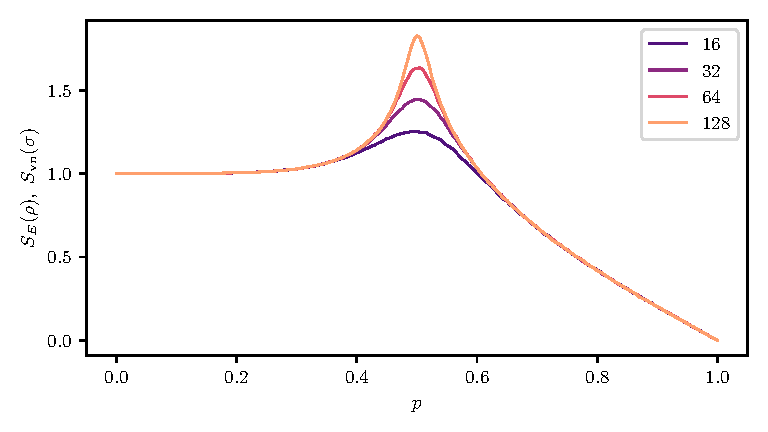
\includegraphics{naive_approach_cleansystem_soloplot.pdf}
  \caption{Cross entropy vs entanglement entropy, no Errors track everything, naive approach (any of them work tho)}
  \label{fig:naive-svn-vs-se-no-error}
\end{figure}

faulty circuit: (naive approach mit fehlern, $\infty$ wird durch $N$ ersetzt)
\begin{figure}[H]
  \centering
  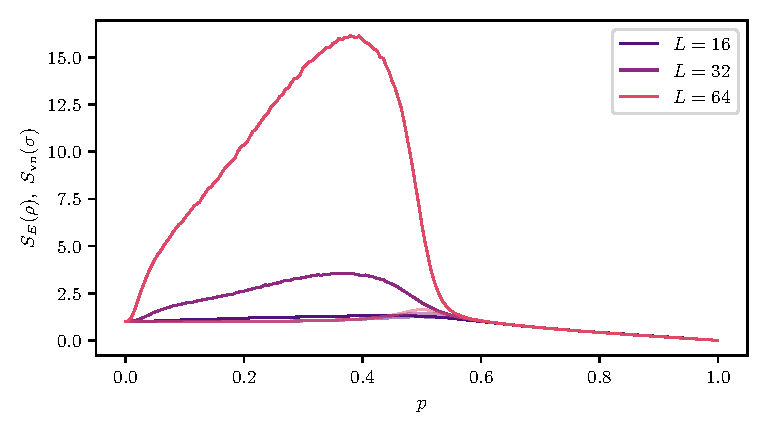
\includegraphics{naive_approach_xerrors_soloplot.pdf}
  \caption{Cross entropy vs entanglement entropy, $X$ Errors track everything,
  naive approach, saller system sizes (this should exists)}
  \label{fig:naive-svn-vs-se}
\end{figure}
\subsection{\enquote{Failure} of the na\"ive approach}

\begin{itemize}
  \item subgroup condition requires errors to be detected (and dealt with in
    some way)
  \item errors which are not succeeded by a measurement will lead to a change
    in the group structure of $S_\rho$ such that $S_\sigma$ \enquote{never has
    the chance to adapt}
  \item maybe we should also implement some ideas from the shadow tomography
    dings, such that errors are circumvented
  \item Undetectable change in group structure happens if an error happens on a
    qubit in a state stabilized by an orthogonal operator, e.g. an $X$-error if
    the qubit is stabilized by $Z$.
  \item The probability of any error happening in the last layer (i.e. after
    all measurements in the circuit happenend) is $1-$ the probability of no
    error, which is given by the binomial distribution
    \[ P(\#\mathrm{err}>0) = 1-\binom{N}{0} (1-q)^N=1-(1-q)^N. \]
  \item For $q=\num{0.01}$ and $N=32$ we have $P\simeq .275$
  \item Of course, this probability says nothing about the actual simulation
    (except for $p=0$) as it could be an error which was preceeded by an $X$
    measurement.
  \item That being said, you could technically compute this probability
    analytically, by going through each layer and multiplying the probabilites
    for \(X\) and not $ZZ$ happening to get the actual probability of failure
   \item This is way too complicated, just to get an estimate on how many
     simulations will end in $\infty$ for \cref{eq:kleins-ineq}. 
\end{itemize}

%Let us now consider the information-theoretic implications of \cref{eq:cross-ent-stab}. 
Recall that the cross entropy is a measure of the quality of an estimate of a
probability distribution \cite{coverElementsInformationTheory2006}. As we are
essentially estimating the experiment, represented by the density matrix
$\rho$, with a uniform probability distribution over the support of $\rho$, the
quality of our estimate depends only on how many events (or in this case,
states) we choose to include in our estimate. In other words, we project onto
an eigenstate $\ket{\phi}$ of $\rho$, where our estimate of the probability of
$\ket{\phi}$ is scaled by how many other states we consider with equal
probability. Alternatively, in the case where the subgroup condition is not
met, we do \emph{not} have $\ket{\phi}$ in $\mathrm{supp}\left( \sigma
\right)$. In this scenario, we project onto the $0$ vector, giving us a
divergent term in the cross entropy.
This also shows how stabilizer
states are particular in that sense. Any stabilizer density matrix we choose
for $\sigma$ will yield this result, independent of $\rho$, as long as $\rho$
is a valid density matrix. 
\section{Other Approaches}\label{sec:other-approaches}
\begin{itemize}
  \item Naive approach fails because of errors, which cannot be detected by
    construction
  \item also, because so far we have only dealt with pure states.
  \item we thus need a new classical post-processsing algorithm
  \item first, we need to disallow errors after the last couple of
    measurements, since these are the ones that make it into the subgroup check
  \item this is, of course, an unphyisical assumption to take, but thats not
    our main concern. informally speaking, we want to test the limits of
    \cref{eq:kleins-ineq} for our system. We found this irreconcilable one in
    the context of our model
  \item if we relax the assumption of errors happening everywhere, we could try
    other approaches and maybe get an idea of how viable the general approach
    of an upper bound is to find a signature of the entanglement transition.
  \item next, we have this condition of diverging cross entropy. Why not go in
    reverse and try an algorithm, which has the stabilizers of $\sigma$ be a
    subgroup of $\rho$.
  \item we can do that by modifying the projections slightly
  \item in the following sections we explore some approaches to modify the
    projection operation to incorporate mixedness
\end{itemize}
\subsection{Minimal Mixing}\label{sec:minimal-mixing}
\begin{itemize}
  \item We would like to compare $\rho$, which is the \enquote{experiment}
    (i.e. a quantum simulator), with $\sigma$, which is the classical
    simulation.
  \item The algorithm follows a similar structure to
    \cite{liCrossEntropyBenchmark2023}, wherein we project the measurement
    outcomes from $\rho$ onto $\sigma$ where it is possible. The difference
    being that we do not start with orthogonal GHZ states, but with identical
    GHZ states. That way, there will be no incompatible measurement as long as
    there are no errors
  \item but what if there are errors?
  \item consider the case that an $X$-error occurred after a $ZZ$-measurement.
  \item Half of the time we will get an incompatible projection, which would
    project onto the zero-vector.
  \item In those cases, we replace the stabilizer by $\mathds{1}$, where the
    incompatibility was detected, instead of replacing it by the measurement
    outcome or the projection.
  \item This ensures that the subgroup condition still holds \emph{and} that
    subsequent measurements on the same site cannot be interfered with, i.e.
    that this qubits stabilizer is $\mathds{1}$ until it gets measured again.
  %\item However, we rolled a nat20 on a sleight of hand skill check: in the
  %  cases, where we \emph{would} get $\infty$, we replace $\sigma$ (whatever
  %  it may be at this point) by $2^{-N} \mathds{1}$
  %\item This is also in line with the general philosophy of the density
  %  matrix. We do not know where the error occurred, and are therefore in a
  %  mixture of all possible quantum states
\end{itemize}
\subsection{Maximal Mixing}\label{sec:maximal-mixing}
\begin{itemize}
  \item the first approach is what we'd call \emph{maximal mixing}.
  \item The maginot line of no errors occuring is still a factor. However, each
    time we encounter a discrepancy for the projections, we remove \emph{all}
    the stabilizers in $\sigma$
  \item since the trivial group is always a subgroup of any group (group
    axioms), we still obey the subgroup rule
  \item the technical details are laid out in \cref{alg:maximal-mixing}
  \item most importantly, for a system with no errors, the bound is perfectly
    saturated, with equality everywhere
  \item when introducing errors, we lose this feature and start to become more
    inaccurate.
\end{itemize}

\section{Results}\label{sec:upperbound-results}
\subsection{Minimal mixing}
\begin{figure}[H]
  \centering
  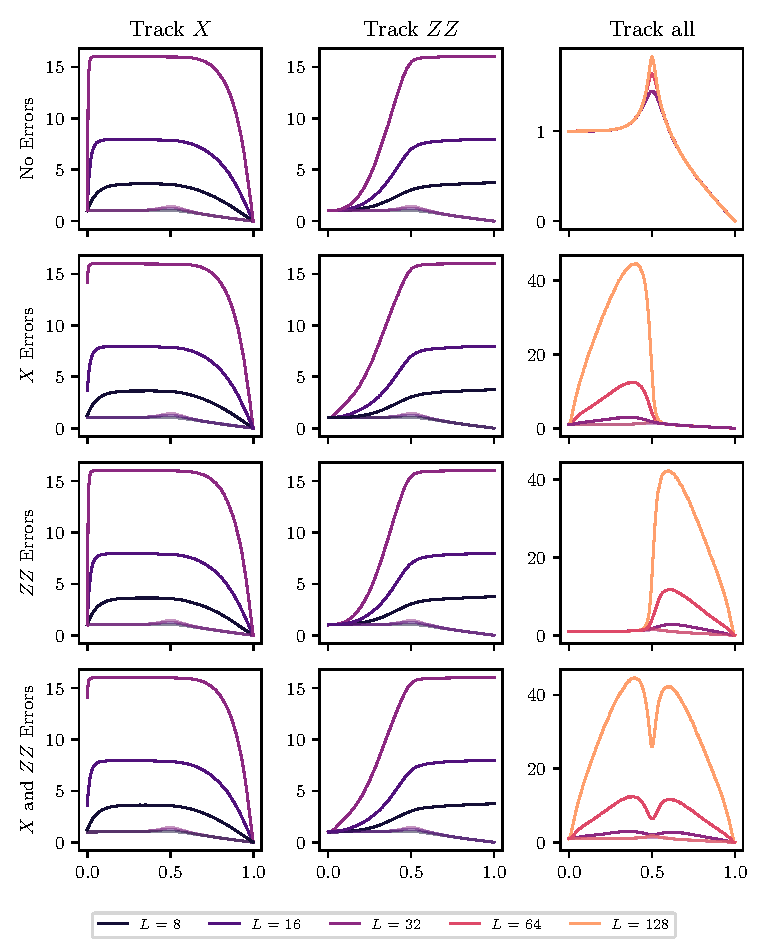
\includegraphics{minimal_mixing-4x3-svn_se.pdf}
  \caption{Cross Entropy and entanglement entropy of selected system sizes with
  periodic boundary conditions. To be able to adequately compare it to LXE the
different trackings and errors are shown in the same manner as in
\cref{fig:err-vs-tra}}
  \label{fig:min_mix-svn_se-4x3}
\end{figure}
\begin{figure}[H]
  \centering
  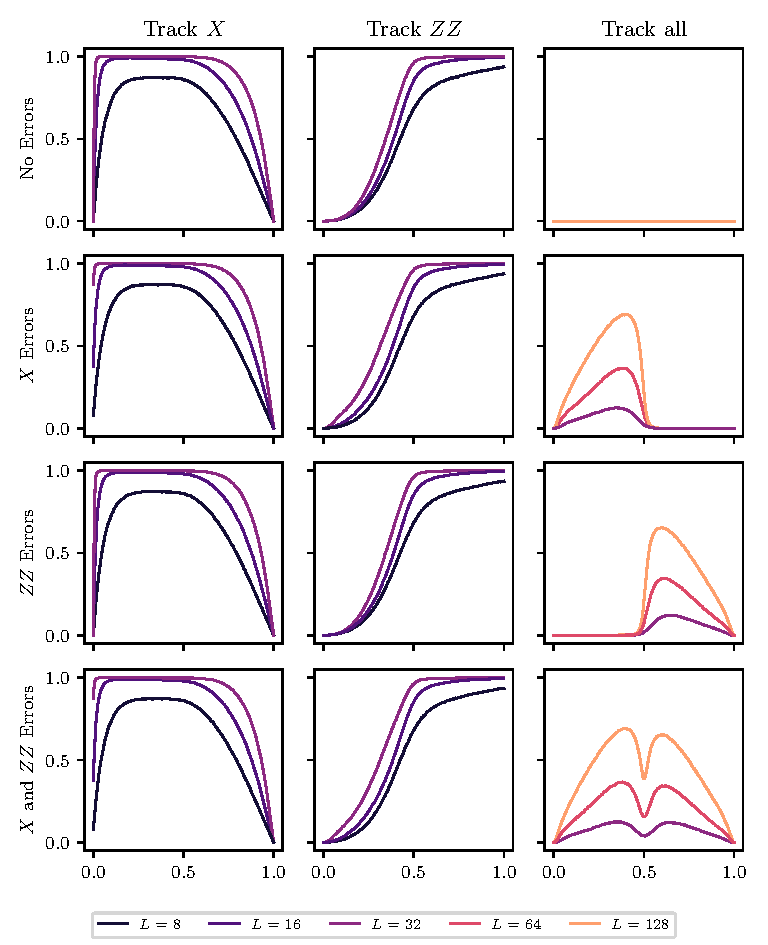
\includegraphics{minimal_mixing-4x3-inftyratio.pdf}
  \caption{Ratio of divergences in cross entropy to number of samples for
    different system sizes
  periodic boundary conditions. To be able to adequately compare it to LXE the
different trackings and errors are shown in the same manner as in
\cref{fig:err-vs-tra}}
  \label{fig:min_mix-inftyratio-4x3}
\end{figure}
\begin{figure}[H]
  \centering
  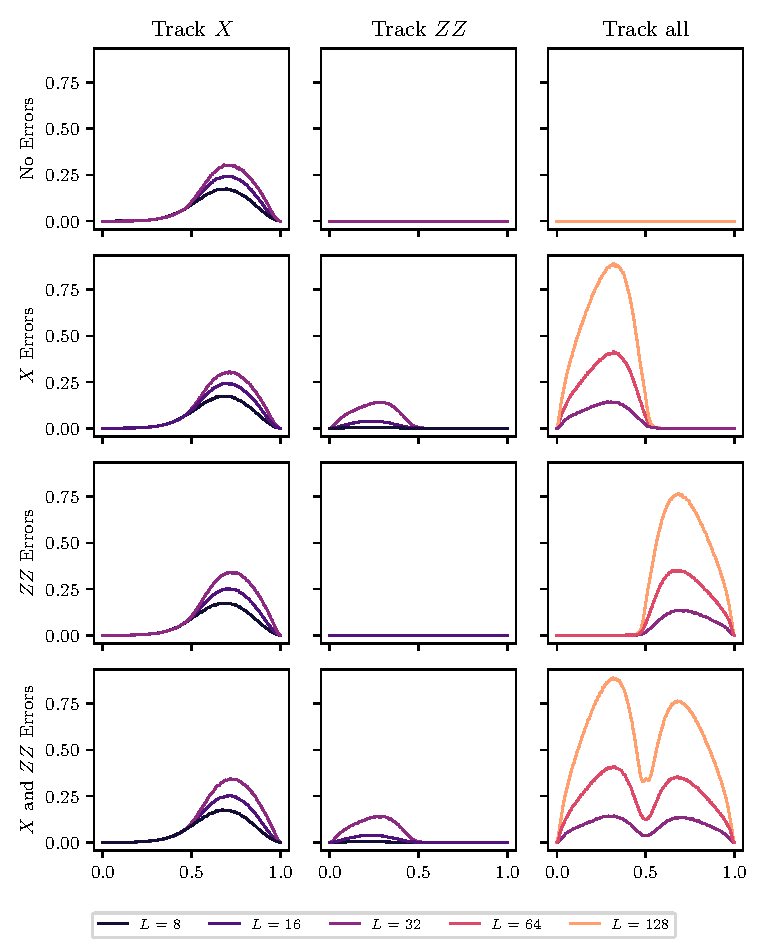
\includegraphics{minimal_mixing-4x3-svn_sigma_full.pdf}
  \caption{$S(\sigma)$ of full density matrix $\sigma$ 
  periodic boundary conditions. To be able to adequately compare it to LXE the
different trackings and errors are shown in the same manner as in
\cref{fig:err-vs-tra}}
  \label{fig:min_mix-svn_sigma_full-4x3}
\end{figure}
\subsection{Maximal mixing}
\begin{figure}[H]
  \centering
  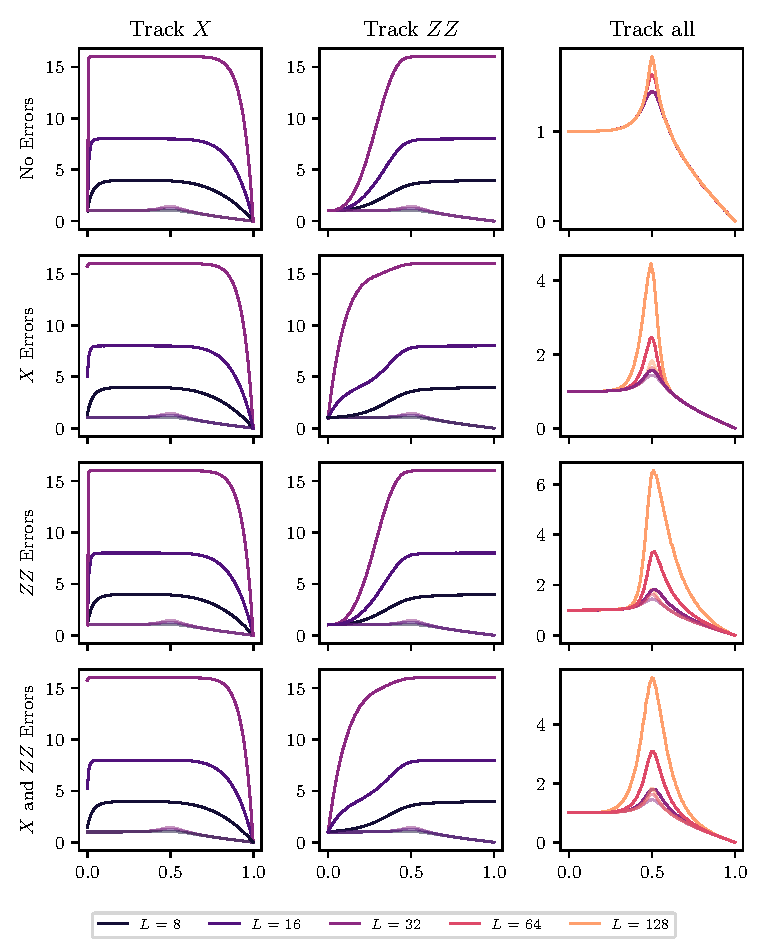
\includegraphics{extreme-rel-ent-4x3-svn_se.pdf}
  \caption{Cross Entropy and entanglement entropy of selected system sizes with
  periodic boundary conditions. To be able to adequately compare it to LXE the
different trackings and errors are shown in the same manner as in
\cref{fig:err-vs-tra}}
  \label{fig:max_mix-svn_se-4x3}
\end{figure}
\begin{figure}[H]
  \centering
  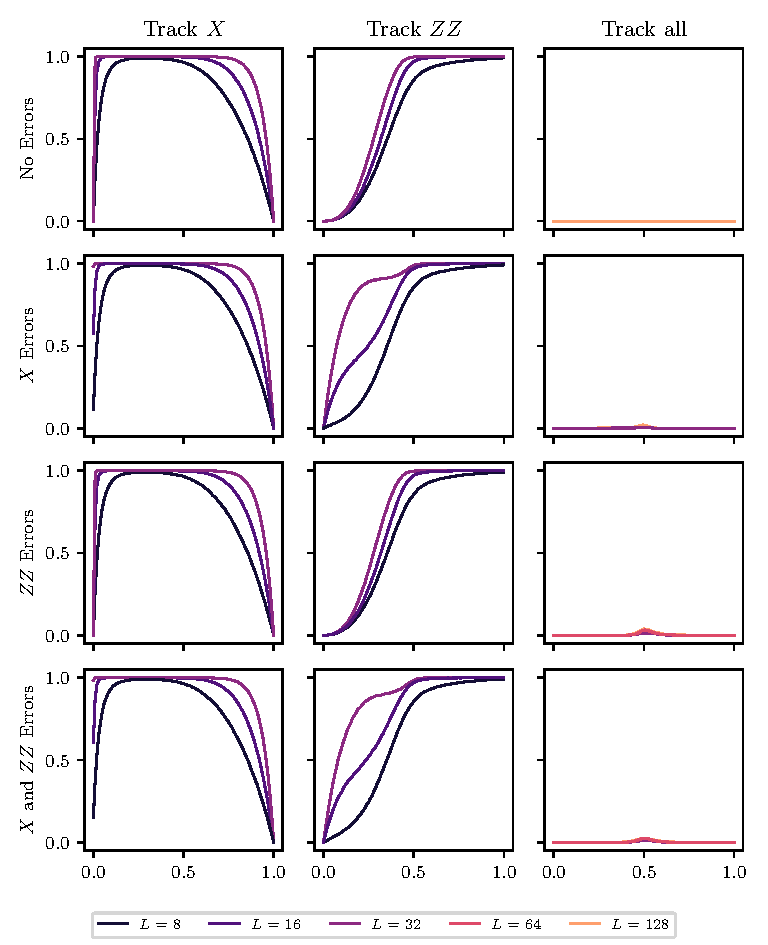
\includegraphics{extreme-rel-ent-4x3-inftyratio.pdf}
  \caption{Ratio of divergences in cross entropy to number of samples for
    different system sizes
  periodic boundary conditions. To be able to adequately compare it to LXE the
different trackings and errors are shown in the same manner as in
\cref{fig:err-vs-tra}}
  \label{fig:max_mix-inftyratio-4x3}
\end{figure}
\begin{figure}[H]
  \centering
  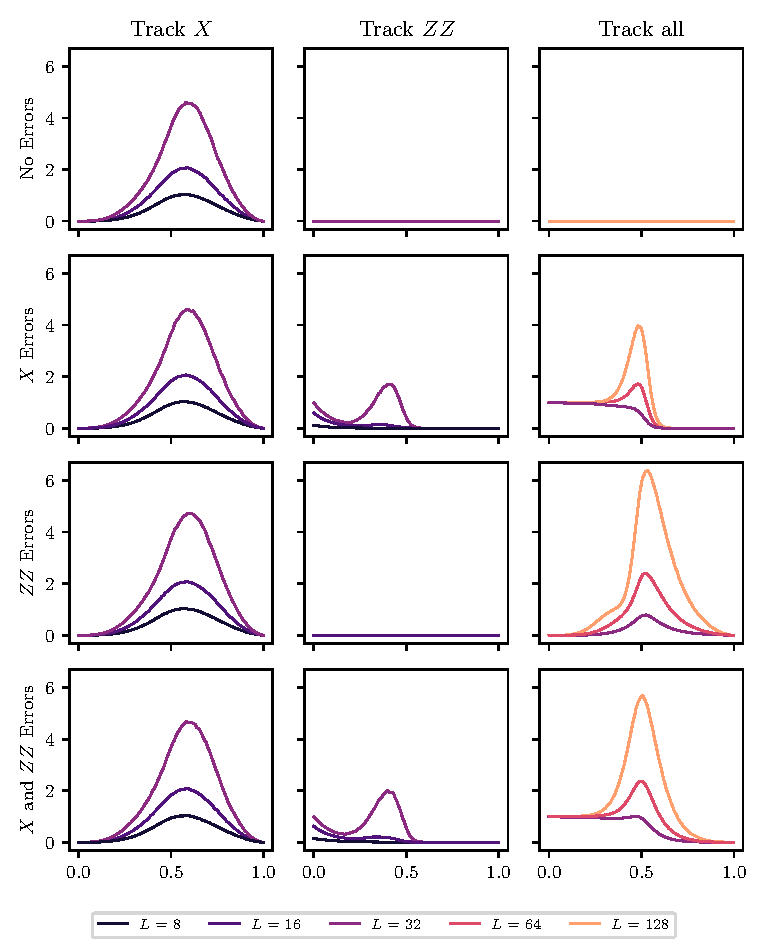
\includegraphics{extreme-rel-ent-4x3-svn_sigma_full.pdf}
  \caption{$S(\sigma)$ of full density matrix $\sigma$ 
  periodic boundary conditions. To be able to adequately compare it to LXE the
different trackings and errors are shown in the same manner as in
\cref{fig:err-vs-tra}}
  \label{fig:max_mix-svn_sigma_full-4x3}
\end{figure}

\section{Regularization}
We can see that, even though we chose our numerical algorithms in a way that
should mitigate the infinities, we still have them. Furthermore, the subgroup
check is a subtle way to incorporate once more what we try to avoid. Namely,
we want to find a density matrix, which is independent of the experimental
density matrix $\rho$. However, with the subgroup check, we implicitly
introduce it into our computation again, as we once more require knowledge of
the full density matrix, bringing us back to the sampling problem. In the
following we present two approaches to regularize the infinity appearing in the
cross entropy. These approaches require nothing but the numerically computed
density matrix $\sigma$. The first approach is one, which could be implemented
in a stabilizer simulator, which has the drawback of being exponentially worse
than the trivial upper bound $N$. The other is more flexible, but lacks an
obvious implementation for stabilizer states. Both of these approaches could be
the subject of further study, as the computational argument is one of
feasibility, but not possibility (i.e., it is possible, but at what
computational cost).
\subsection{Exponential Ansatz}
For the first regularization we choose an exponential Ansatz. The basic reasoning
behind this Ansatz is twofold. First, we want to ensure that the support of
$\sigma$ is large enough to contain the support of $\rho$. That is, what we
failed to achieve numerically, we attempt to achieve analytically, while
ensuring that the classical processing step is only a function of the
measurement out comes, $\sigma \equiv \sigma(\mathbf{m})$, and not the density
matrix, which we implicitly had by checking the subgroup condition on each run.

The second reason for this Ansatz in particular is the computability. Since we
are performing classical computations via the stabilizer formalism, we reduce
the memory requirements significantly. Storing a state of an $N$ qubit Hilbert
space is done in quadratic space complexity (cf. \cref{ch:mixed}). If we were
to write out the density matrix of, e.g., $N=100$ qubits explicitly, we would
be faced with an exponentially large matrix. If we chose $\sigma$ arbitrarily,
we would be faced with the herculean task of diagonalizing a $2^{100} \times
2^{100}$ matrix, way beyond the scope of any reasonable computational
feasibility. By exponentiation we ensure that the logarithm \enquote{gets eaten
up} such that we are dealing with the density matrix itself. 

As mathematical expression we may write
\begin{align}
  \tilde{\sigma} = \frac{\exp[\sigma]}{\Tr[\exp[\sigma]]}
.\end{align}
Substituting $\tilde{\sigma}$ back into the right hand side of
\cref{eq:kleins-ineq} we get
\begin{align}
  -\Tr[\rho\log\rho]\leq-\Tr[\rho\log\tilde{\sigma}] = -\frac{1}{\ln 2}\Tr[\rho\sigma] +
  \log(\Tr[\exp[\sigma]])
\end{align}

By choosing this Ansatz we effectively recover the Cauchy-Schwarz inequality

In summary, we have a measurement record $\mathbf{m}$, obtained from running an
experimental circuit $C$ on $N$ qubits. This measurement record gets piped into
a classical simulator so that we can compute the upper bound (cf.
\cref{eq:kleins-ineq}). 
$\Tr[\rho\log\sigma]$. 
%We are interested in the half-system
%entanglement entropy, $$-\Tr[\rho_A \log \rho_A]\qquad{\text{with}}\qquad
%\rho_A = \Tr_B[\dyad{\phi_\mathbf{m}}]$$, where $A$ and $B$ refer to the two
%halves of the system. 
We then pipe the measurement record to a classical
simulator 
\begin{align}
  \tilde{\sigma} = \frac{e^\sigma}{\Tr[e^\sigma]}
.\end{align}

we still have a valid density matrix, given we normalize appropriately. 
condensed into . If we were to write out an $N$ qubit
density 
Second, and more importantly for this Ansatz in particular, we

Thus, we prepare $\sigma(\mathbf{m})$ by means of classical reconstruction,
with either one of the previous numerical algorithms. Here, since we 
\subsection{Rescaling probabilities}
\begin{align}
  D_\sigma = \mqty(\dmat{1-\varepsilon,1-\varepsilon,\ddots,\varepsilon,\varepsilon})
.\end{align}
\section{Summary}

\clearpage
\section{some relevant references}
\begin{enumerate}
  \item \textcolor{red}{\citetitle{aaronsonImprovedSimulationStabilizer2004}
      fuck why didn't i read it in its entirety earlier: section 7 does the
    job\ldots}
  \item \citetitle{veitchResourceTheoryStabilizer2014}, entropic quantities of
    magic states; quantifying non-stabilizerness. This paper is with gottesman
    himself, so i thought it might be interesting to study. 
  \item \citetitle{niekampEntropicUncertaintyRelations2012}, more or less what
    it says. No regularization scheme or whatever. I think stabilizers are
    mentioned tangentially, thats why i found it.
  \item \citetitle{lashkariRelativeEntropiesConformal2014}, $\leftarrow$ me
    grasping for straws.
  \item \citetitle{leonePhaseTransitionStabilizer2024}, very recent, not too
    particularily relevant to our stuff as far as i can tell.
  \item \citetitle{wuEntanglementUpperBound2011} idfk\ldots
  \item \citetitle{vedralEntanglementMeasuresPurification1998} one of the more
    promising papers i've come across. probably helpful in proving the failure
    of the na\"ive approach. However, it was published in 1998. It most likely
    has nothing to do with stabilizers.
  \item \citetitle{lindenQuantumEntropyCone2013}, probably some interesting
    stuff in there, but not the thing i want.
  \item \citetitle{buExtremalityStabilizerStates2024}, this paper is where most
    of my confusions come from. 
\end{enumerate}
